\section{Learning a default strategy}
\label{sec:part2}
In the previous chapter we created a calculator which can calculate the probability of winning with any hole cards in any game state. We will use the calculator in this section to estimate the strength of our hole cards.\\

Before we can learn our poker bot to adapt to opponents strategy we first need it to learn a default one. When the poker bot first joins a poker game it has no information about the opponent. In this case it must use a default strategy while it gathers more information.

In this chapter we will find a solution to the problem statement:

\vspace{4mm}
\begin{statementBox2}{Problem statement 2}
How can we develop a default strategy without having information about the opponents?
\end{statementBox2}
\vspace{4mm}

Because the default strategy has to work against any type of opponent, we don't expect it to be able to win against every type of opponent. The focus of the default strategy is not to make the poker bot win, although that would be preferable, its goal is instead to reduce the loses while the system gathers information about the opponent. But how can we make sure that we create a bot that plays on a sufficient level that it wont loose unnecessary?

\subsection{Design}
To develop a default strategy we have two options.

The first option is to directly program how the computer shall act in all situations. In this case the programmers need a deep insight in how to play poker in order to decide what decisions are optimal in the different situations. One can also use the expertise of professional poker players in case one lack the insight.

The second option is to develop an self-learning algorithm for the computer. Such an algorithm uses the concept \textit{watch and learn} by observing other players playing poker and trying to learn the strategy behind the decisions. This method requires that the computer has something to observe.

Since we do not have any particular insight in how to play poker and do not have expertise from any pro poker players, we will implement a self-learning algorithm. Another advantage by using this method is that the computer is not limited by our understanding of the game instead it might end up learning things we did not know beforehand.

The University of Alberta has a research group that specializes in field of artificial intelligence in poker. They have released a dataset containing data from ~18.000 real-life rounds of Texas hold'em limit poker. The dataset only contains the hole cards of the players who make it to the showdown, so there is no data about the hole cards of the players who folds. This data will be used to develop the default strategy.\\

To implement the self-learning algorithm we use an artificial neural networks (ANN), see section \ref{sec:nn}. Our algorithm needs to recognise patterns in the players decisions and ANNs are very good at this. \\

We use an iterative development method to design the ANN for the algorithm. We start by designing a simple ANN and then move on to more complex ANNs.

\subsubsection{Artificial neural network (ANN)}
\label{sec:nn}
An artificial neural network (ANN) inspired by the human brain. It is well suited for finding an approximation to a non-linear function. An ANN can take any number of inputs and return any number of outputs. 

An ANN is made up of neurons that are connected into a network. Each neuron takes a set of inputs and give one output. The output of a neuron is sent to the connected neurons. Each input has a weight that determines influence of the input. The neuron uses an input function to calculate the net input, usually the sum of all weighted inputs, and pass it on to the transfer function. The type of transfer function determines the output. A step function return zero or one if the net input is above a certain threshold. This is useful for logical functions. If one need a value between zero and one a sigmoid function can be used instead.

\begin{figure}[H]
  \center
    \includegraphics[scale=0.4]{images/nn/neuron.png}
  \caption{Model of a neuron. \label{fig:neuron}}
\end{figure}

An ANN consists of three types of layers as shown in figure \ref{fig:mlp}. The coloured circles are neurons and the arrows shows the connections between the neurons. It will always contain an input layer and an output layer but it can contain any number of hidden layers. The simplest type of ANN is the perceptron and is used for a single calculation. It consists of only an input layer and an output layer but no hidden layers. A multilayer perceptron also includes hidden layers and is used for more complex domains with multiple layers of computations.

\def\layersep{2.5cm}

\begin{figure}[H]
\center
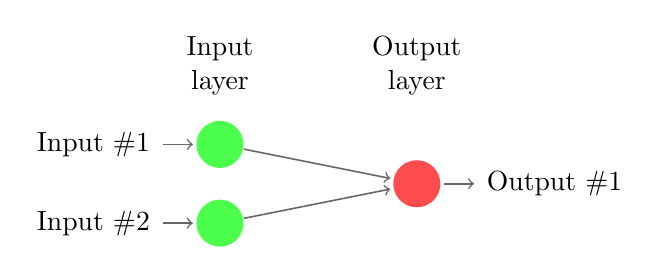
\begin{tikzpicture}[shorten >=1pt,->,line width=0.2mm,draw=black!60, node distance=\layersep]
    \tikzstyle{every pin edge}=[<-,shorten <=1pt]
    \tikzstyle{neuron}=[circle,fill=black!25,minimum size=17pt,inner sep=0pt]
    \tikzstyle{input neuron}=[neuron, fill=green!70];
    \tikzstyle{output neuron}=[neuron, fill=red!70];
    \tikzstyle{hidden neuron}=[neuron, fill=blue!70];
    \tikzstyle{annot} = [text width=4em, text centered]

    % Draw the input layer nodes
    \node[input neuron, pin=left:Input \#1] (I-1) at (0,-1) {};
    \node[input neuron, pin=left:Input \#2] (I-2) at (0,-2) {};

    % Draw the output layer node
    \node[output neuron,pin={[pin edge={->}]right:Output \#1}] (O-1) at (\layersep,-1.5) {};

    % Connect every node in the input layer with every node in the
    % hidden layer.
    \path (I-1) edge (O-1);
    \path (I-2) edge (O-1);

    % Annotate the layers
    \node[annot,above of=I-1, node distance=1cm] (il) {Input layer};
    \node[annot,right of=il] {Output layer};
\end{tikzpicture}
\caption{Perceptron with two inputs and one output. \label{fig:perceptron}}
\end{figure}
\vspace{4mm}
\input{other/models/multi-perceptron.tex}

The ANN can be trained using a training set of inputs. Using supervised learning, in contrast to unsupervised learning, one must also supply an expected output. The ANN starts with random values for all the weights. Backpropagation is the most common supervised learning method. For each input it will adjust the weights in order to get closer to the expected output. It will continue doing this until the outputs are close enough to the expected outputs.

The ANN can be validated afterwards. This is done using a test set different from the training set.

\subsubsection{First ANN design}
For our first attempt we design a simple perceptron. The perceptron takes two inputs, and gives two outputs. 

The first input is the hand strength. We use the calculator from section \ref{sec:part1} to calculate the probability of winning from the hole cards and community cards against one opponent. The reason we always find the probability against a single opponent is because the probability of winning decreases drastically as the number of opponents increases. We use the absolute hand strength rather than a hand strength relative to the number of players. 
This makes it easier to compare the hands strengths in situations with a different number of players. The number of players is instead the second input.

The first output is whether or not to be defensive by checking or calling. The second output is whether or not to be aggressive by betting or calling. The outputs will both be zero in case it is best to fold. 
The perceptron uses a step function as transfer function in both output neurons.

\def\layersep{2.5cm}

\begin{figure}[H]
\center
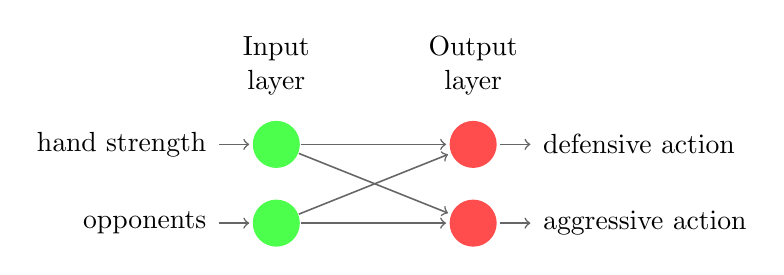
\begin{tikzpicture}[shorten >=1pt,->,line width=0.2mm,draw=black!60, node distance=\layersep]
\tikzstyle{every pin edge}=[<-,shorten <=1pt]
    \tikzstyle{neuron}=[circle,fill=black!25,minimum size=17pt,inner sep=0pt]
    \tikzstyle{input neuron}=[neuron, fill=green!70];
    \tikzstyle{output neuron}=[neuron, fill=red!70];
    \tikzstyle{hidden neuron}=[neuron, fill=blue!70];
    \tikzstyle{annot} = [text width=4em, text centered]
    

    % Draw the input layer nodes
    \node[input neuron, pin=left:hand strength] (I-1) at (0,-1) {};
    \node[input neuron, pin=left:opponents] (I-2) at (0,-2) {};

    % Draw the output layer node
    \node[output neuron,pin={[pin edge={->}]right:defensive action}] (O-1) at (\layersep,-1) {};
    \node[output neuron,pin={[pin edge={->}]right:aggressive action}] (O-2) at (\layersep,-2) {};

    % Connect every node in the input layer with every node in the
    % hidden layer.
    \path (I-1) edge (O-1);
    \path (I-2) edge (O-1);
    \path (I-1) edge (O-2);
    \path (I-2) edge (O-2);

    % Annotate the layers
    \node[annot,above of=I-1, node distance=1cm] (il) {Input layer};
    \node[annot,right of=il] {Output layer};
\end{tikzpicture}
\caption{First ANN design. \label{fig:nn1}}
\end{figure}

This approach did not seem to suit our needs as after training the neural network it did not make reasonable decisions. The neural network somewhat found a context between the number of opponents versus as to if we should be aggressive or not. The probability of the player having the winning hand did not weight as much as the number of opponents did. Therefore we chose to implement a more complex neural network as the results from the perceptron perhaps were not the most preferable decisions in the given situations.\\

\subsubsection{Second ANN design}
A multi-layer-perceptron(will be refereed to as MLP) is closely related to our first described perceptron. The most simple structure is almost identical, but instead only having 2 layers, the input and output layers. The MLP can have multiple hidden layers inbetween the two layers of inputs and outputs.
The inputs in the MLP is taking the same as the earlier discussed perceptron, but also the chips the current player has, how much it will cost the player to call the current bid, and the total pot(a.k.a the profit) for that game state.
The MLP has 1 hidden layer with 2 hidden neurons. One hidden neuron for the probability of having the winning hand and the number of opponents. The second hidden neuron is for the chips, the cost and the pot.
As with the perceptron the sum of each weight in the MLP will be passed into a transfer function. In this case we chose to use a STEP function.

\input{other/models/default-nn2.tex}

\subsection{Test}
To test our first simple neural network a.k.a the perceptron, we ran through x games in the dataset. The neural network is not able to get particular smarter when running through an additional set of entries as the data is from different players and x games should be sufficient for the neural network to gain some kind of knowledge on how to play as the goal of this strategy is not to have a bot that can beat the opponents but minimize the loses.
The neural network now had to learn from the dataset 

\subsection{Discussion}
When our artificial intelligence starts out by playing the games of poker it doesn't have any kind of information about the opponents. So to make sure that the bot wont just go keep throwing away the bank roll. Instead we wanted the bot to minimizes our losses so that we would still have a decent bank roll when we have gathered information about the opponents so that the bot could make qualified guesses at what move would be the most appropriate in terms of the current opponent. The default player was never meant to be on the same level as a human player, but humans are only in a slightly better position than the default bot. The human player can like the bot only see the hole and community cards, but a human is also able to make a profile of the bot in their head. This means that they can learn how the bot decides and exploit this. 
This is one of the reasons that we chose to go with a neural network. In a neural network we are able to of course train the network to make correct decisions based on the targeted output that we give it.
But as the game proceeds the neural network has an input which will weight when we have enough information about the opponents to shift our gameplay from the default play style to a more adaptive one.
The time that it takes a human player to learn about the bot and adapt to it, should be the same for the bot. So if we imagine a human player who is good enough to decipher the way the bot is playing and adapt to it. When the human player does that, the bot should also have started to change its ways. Slowly as the bot learn it will adapt more and more to the opponent so when we have enough information the bot will shift completely and disregard the default play style.
\subsection{Conclusion}